\documentclass[11pt]{article}

\usepackage[utf8]{inputenc}
\usepackage[T1]{fontenc}
\usepackage{lmodern}
\usepackage[margin=1in]{geometry}
\usepackage{amsmath, amssymb}
\usepackage{microtype}
\usepackage{enumitem}
\usepackage{xcolor}
\usepackage{tikz}
\usetikzlibrary{positioning, fit, arrows.meta, calc, backgrounds, shapes.geometric}
\usepackage{booktabs}
\usepackage{array}
\usepackage{pifont}
\usepackage[round]{natbib}
\usepackage{hyperref}
\hypersetup{colorlinks=true, linkcolor=black, urlcolor=blue, citecolor=black}

% Convenience macros.
\newcommand{\anchorW}{W_{\text{anchor}}}
\newcommand{\anchorB}{b_{\text{anchor}}}
\newcommand{\Lewc}{L_{\text{EWC}}}
\newcommand{\Ltask}{L_{\text{task}}}
\newcommand{\reff}{r_{\text{eff}}}
\newcommand{\ac}{\text{ac}}
\newcommand{\R}{\mathbb{R}}
\newcommand{\arm}[1]{\texttt{#1}}
\newcommand{\headline}{$\bigstar$}

\title{Trioron: an epigenetic-inspired self-organizing architecture\\
       for resource-bounded continual learning}
\author{Marcelinus R.\ Hatorangan%
        \thanks{Correspondence: \texttt{adeussinca@gmail.com}.
                Repository: \url{https://github.com/Marcrockhat/trioron-project}.}}
\date{2026-05-08}

\begin{document}
\maketitle

\begin{abstract}
We describe a small neural-network architecture in which each node carries
three coupled state variables --- weight, plasticity, and utility --- and
in which growth, pruning, regularization, and offline consolidation are
coupled to a per-node resource budget. The architecture combines
established components --- elastic weight consolidation, capacity-expanding
layers, episodic and storage-free pseudo-rehearsal, and mixed-precision
deployment --- with a stress-driven plateau detector and a
sleep-time consolidation pass. On a 30-class class-incremental benchmark
(\emph{chained-15}) at $\approx 8\,$K trainable parameters we report
results comparable with, but not uniformly better than, strong baselines
from the regularization, partition, and rehearsal families; the deployment
target is a $\sim$157~KB checkpoint that can be shipped, woken on new
data in the field, and re-shipped with prior tasks preserved at $\geq
0.95$ task-aware accuracy. We do not claim a fundamentally new continual-
learning mechanism. Our contribution is a system-level integration of
known mechanisms --- with a small biological framing that motivates the
particular couplings --- and an evaluation under bounded-memory deployment
constraints that the named baselines were not designed to address. All
results are $n = 3$ multi-seed; we are explicit about where this scale
limits the conclusions.
\end{abstract}


\section{Introduction}
\label{sec:intro}

A neural network that grows as it learns is not a new idea. Foundational
work spans the constructive-networks line --- Cascade-Correlation
\citep{fahlman1990cascade}, the Upstart algorithm \citep{frean1990upstart},
self-organizing topographic maps \citep{kohonen1982som} --- as well as
more recent capacity-expanding architectures: Progressive Networks
\citep{rusu2016progressive}, Net2Net \citep{chen2016net2net}, and
Dynamically Expandable Networks (DEN) \citep{yoon2018den}. The recurring
intuition is that learning-as-growth, rather than
learning-as-allocation-within-a-fixed-budget, better matches what
biological systems do. With the rise of large language models, interest
in adaptive systems has surged, but most LLMs are trained with massive
central-resource budgets, which limits the practicality of tailoring such
models to individual users on commodity devices.

A second line of work tackles the same problem from the opposite side.
Methods such as PackNet \citep{mallya2018packnet}, HAT
\citep{serra2018hat}, EWC \citep{kirkpatrick2017overcoming}, and Online
EWC \citep{schwarz2018progress} operate within a fixed parameter envelope
and partition that envelope across tasks --- by mask-based isolation, by
hard attention, or by quadratic anchoring on the weights estimated as
important for prior tasks. While each is effective at moderate task
counts, all share the same saturation regime: when the envelope fills,
new tasks are accommodated only by overwriting prior knowledge or by
routing through increasingly compromised mask intersections. Biological
systems, by contrast, operate under hard physical bounds (finite cranial
volume) yet continue to learn throughout life --- suggesting that
\emph{growth, pruning, and remodeling} are part of the answer rather
than allocation alone.

The capacity-expanding family addresses growth but typically not the
\emph{cost} of growth: there is no built-in mechanism for the network to
decline a proposed expansion that would exceed available resources, nor a
graceful degradation pathway when resources become scarce. Learning
capacity is implicitly assumed to be supplied by the deployment
environment rather than negotiated with it. Closing that gap is one of
the design motivations of this work: a network that knows when not to
grow even if growth would help, and that has a sleep-time pathway for
freeing substrate by consolidating what is already stable.

We borrow design metaphors from cellular biology rather than claiming
biological realism. During development, individual cells establish their
identity through epigenetic mechanisms driven by spatial gradients of
signaling molecules \citep{wolpert1969positional}. As cells divide,
epigenetic marks such as DNA methylation \citep{smith2013dna} and histone
modifications \citep{bannister2011histone} act as cellular memory ---
which genes are accessible for transcription and which are silenced ---
and these marks are inherited across mitosis \citep{allis2016hallmarks}.
Small non-coding RNAs (microRNAs) act as a separate, faster regulatory
layer \citep{bartel2009micrornas}: produced and consumed in stoichiometric
pools, they post-transcriptionally regulate plasticity-related gene
expression in concentration-gradient-dependent ways
\citep{schratt2009micrornas} and have been implicated in the sleep-driven
synaptic-homeostasis cycle that consolidates new learning while pruning
weak connections \citep{tononi2014sleep}. The architecture in
\S\ref{sec:methods} borrows three of these mechanisms --- anchoring
(methylation), stress-responsive plasticity modulation (HPA-axis-style
modulation), and resource-limited consolidation pools (small-RNA-style
throttling) --- as design metaphors that motivate specific implementation
choices. We do not claim mechanistic fidelity beyond the metaphor.

Work on cultured-neuron substrates has shown that biological neurons can
be trained to play a simple video game (Pong) under a coordinated
reward-and-penalty stimulation protocol \citep{kagan2022dishbrain}. We
take this as informal evidence that \emph{cellular-level} mechanisms
(rather than synapse-level alone) are a viable design direction; we do
not import the Kagan~et~al.\ protocol or claim a biological-validity
result of our own.

\paragraph{Contribution and scope.}
We propose a tri-parametric node --- the \emph{trioron} --- and an
architecture that aggregates such nodes into networks capable of
autonomous expansion and continual learning under bounded resources. The
architecture is targeted at the regime where computational and memory
budgets are constrained but the requirement for continual adaptation is
high: agentic AI applications, IoT and embedded systems, and personal
devices that must grow alongside their user rather than be replaced when
the user's needs evolve. In such environments, the model specializes to
its user's specific context rather than serving as a generic system.
Through continual interaction it acquires representations that reflect
individual usage patterns --- recurring vocabulary, environmental cues,
characteristic tasks --- and integrates these into its growing internal
structure without requiring centralized retraining.

We do not claim the trioron is a new continual-learning mechanism. The
contribution is the \emph{integration}: per-node plasticity coefficients
attached to EWC, a stress-driven plateau detector that scales the task
loss but not the regularizer, a sleep-time replay-and-purge pass with a
strict per-cycle event cap, a storage-free pseudo-rehearsal scheme that
summarizes each past class as $(\mu_c, \sigma_c)$ in a frozen-projection
code space, and a two-phase row-archive plus int8 quantization path that
turns shipping into a controlled handoff. We benchmark this assembly
against five named continual-learning families on a 30-class
class-incremental benchmark and report where it wins, where it ties, and
where it loses.

\paragraph{Honest limits.}
All multi-seed results in this paper are $n = 3$. The benchmark is small:
30 to 46 classes drawn from MNIST, Fashion-MNIST, and EMNIST-letters at
an MLP-head joint-training ceiling of $\approx 0.93$ for the 46-class
union. We do not attempt CIFAR-class-incremental or LLM-scale evaluation,
and we do not extrapolate beyond what we measured. The defensible pitch
is not ``we beat all continual-learning methods'' --- it is ``we exhibit
performance comparable with the continual-learning baselines on a class-
incremental benchmark, while occupying a $\sim$157~KB deployment regime
that those baselines were not designed for.''

\paragraph{Disclosure.}
This work was carried out in collaboration with two personified AI
assistants: \emph{Gemma} (a Gemini-Pro instance acting in an
academic-advisory role) and \emph{Chloe} (a Claude Opus 4.7 1M-context
instance acting in an engineering role). The collaboration was structured
as iterative design dialogue --- human-led problem framing and final
decision-making, AI-supported implementation, analysis, and writing.
The human author holds sole responsibility for all claims, methodological
choices, and interpretations. We disclose this collaboration following
recent editorial guidance \citep{nature2023chatgpt, zielinski2023wame},
which permits AI-assisted contributions but explicitly excludes AI
systems from being listed as authors of record.


\section{Related Work}
\label{sec:related}

The architecture described here sits at the intersection of four
established lines of work: capacity-expanding networks, regularization
and partition methods for continual learning, rehearsal-based methods,
and modular composition. None of these families is being reinvented;
the contribution of this work is in their coupling and in the
deployment regime targeted.

\subsection{Capacity-expanding networks}
\label{sec:rel-cap}

Cascade-Correlation \citep{fahlman1990cascade} and the Upstart algorithm
\citep{frean1990upstart} are early constructive-network methods that grow
hidden units one at a time, stopping when an error criterion is met.
Self-Organizing Maps \citep{kohonen1982som} grow a topographic map in
which neighboring units share representational locality. Progressive
Networks \citep{rusu2016progressive} add a frozen task-specific column
per task with lateral connections to prior columns, preserving prior
knowledge by construction at the cost of a per-task parameter footprint.
Net2Net \citep{chen2016net2net} grows a network width-wise and depth-wise
in a function-preserving way, used to accelerate training rather than to
expand capacity in a continual-learning setting.

DEN \citep{yoon2018den} is the closest precedent for our growth path: it
selectively re-trains, expands, and splits hidden units when new tasks
are encountered. Our growth trigger differs in being conditioned jointly
on a loss plateau, a rank-saturation signal computed from latent
singular values, and a gradient-stability check
(\S\ref{sec:structural-plasticity}); growth is then gated against a
per-curriculum byte budget. The shared limitation across this family is
that growth is ungated by an explicit cost model. Our design adds the
budget pre-flight check and a sleep-time pathway for freeing substrate
when growth is denied.

\subsection{Continual learning under a fixed envelope}
\label{sec:rel-cl}

Regularization-based methods anchor weights estimated as important for
prior tasks: EWC \citep{kirkpatrick2017overcoming} uses a per-weight
quadratic Fisher penalty; Online EWC \citep{schwarz2018progress}
accumulates Fisher across tasks; Synaptic Intelligence
\citep{zenke2017si} replaces Fisher with an online importance estimate;
Memory Aware Synapses \citep{aljundi2018mas} estimates importance from
output sensitivity. Partition-based methods isolate per-task subspaces:
PackNet \citep{mallya2018packnet} prunes and reuses; HAT
\citep{serra2018hat} learns hard binary attention masks. Distillation
methods such as Learning without Forgetting \citep{li2018lwf} keep an
older copy of the network as a soft target on old-class columns.

We use EWC with per-node plasticity coefficients
(\S\ref{sec:ewc-substrate}) as the regularization substrate, and we
benchmark against Online EWC, PackNet, HAT, and LwF$+$EWC as
named-family competitors (\S\ref{sec:competitor-sweep}). The novel
element is not the regularizer but how it interacts with growth, with
the dream-time event cap, and with the dream archive: nodes that have
settled their Fisher and stopped contributing gradient become
\emph{archived} (\S\ref{sec:archive}) rather than indefinitely
regularized.

\subsection{Rehearsal and pseudo-rehearsal}
\label{sec:rel-rehearsal}

Episodic-replay methods store past samples directly: GEM
\citep{lopezpaz2017gem} maintains an episodic memory of past examples
and projects gradients to remain consistent with it. We use a hippocampal
buffer with $K \in \{1, 10, 20, 50\}$ samples per past class as the
episodic-rehearsal baseline (\S\ref{sec:replay}). Generative-replay and
data-free methods avoid the storage cost: DeepInversion
\citep{yin2020deepinversion} synthesizes proxy training data by
optimizing an input toward a desired logit configuration. We use
DeepInversion-style code synthesis as a tested-and-rejected baseline
(\S\ref{sec:manifold-replay}, \S\ref{sec:pareto}); the ``manifold
replay'' scheme we use instead summarizes each past class as a small
diagonal-Gaussian sketch in the network's first-hidden-layer code space.
The mechanism is a pseudo-rehearsal scheme rather than a new
distillation method; the contribution is that storing $(\mu_c,
\sigma_c)$ in a \emph{frozen} projection space matches a $K = 20$
episodic buffer at one-tenth the storage on the benchmark we test.

\subsection{Modular and mixture-of-experts composition}
\label{sec:rel-modular}

Branch-Train-Merge \citep{li2022btm} and Branch-Train-Mix
\citep{sukhbaatar2024btx} train independent expert language models on
disjoint domains and merge them, either by parameter averaging or by
training a gating network. Expert Gate \citep{aljundi2017expert} routes
inputs to the right expert via a per-expert generative model. Our
multi-branch absorption (\S\ref{sec:absorption}) is closest to Expert
Gate: branches share a frozen random projection (the \emph{shared-seed
invariant}, see \S\ref{sec:absorption}), and the per-class manifold
sketch already produced for pseudo-rehearsal serves as the analytic
gate. The novel element is not the routing mechanism but that the gate
re-uses storage that the rehearsal pathway already maintains, and that
absorption requires no fusion-layer training.

\subsection{Biological inspiration}
\label{sec:rel-bio}

We borrow language and design metaphors from epigenetics
\citep{wolpert1969positional, smith2013dna, bannister2011histone,
allis2016hallmarks, bartel2009micrornas, schratt2009micrornas,
tononi2014sleep} and from in-vitro cultured-neuron experiments
\citep{kagan2022dishbrain}. We are explicit that these are metaphors
and that the architecture's mechanisms are ML mechanisms; the
biological framing motivates which couplings to try, not which
mechanisms to claim.


\section{Methods}
\label{sec:methods}

\paragraph{Notation.}
$n$ is the number of nodes in a layer; $d$ is the layer's incoming
dimension; $B$ is batch size; $t$ indexes tasks in a curriculum.

\subsection{The Trioron Node}
\label{sec:trioron-node}

A \emph{trioron} is a single computational unit characterized by three
coupled state variables, generalizing the standard artificial neuron:

\begin{itemize}[leftmargin=1.5em]
  \item $w \in \R^{d}$ --- incoming weights (a row of the layer's weight
        matrix).
  \item $\lambda \in \R_{\geq 0}$ --- per-node \emph{plasticity coefficient}:
        a per-unit scalar that scales the unit's contribution to the
        elastic-weight consolidation (EWC) penalty. Larger
        $\lambda \Rightarrow$ stiffer; smaller $\lambda \Rightarrow$ more
        plastic.
  \item $u \in \R$ --- per-node \emph{utility score}: a running estimate
        of the unit's contribution to the network's outputs. Used as the
        signal for pruning decisions (cells with persistently low $u$
        are candidates for removal).
\end{itemize}

A \emph{trioron layer} aggregates $n$ trioron nodes that share an incoming
dimension. We hold the per-node state in vectors $\lambda, u \in \R^{n}$
and a weight matrix $W \in \R^{n \times d}$ where row $i$ is $w_i$. The
forward pass for input batch $X \in \R^{B \times d}$ is
\begin{equation}
  H = \sigma\!\bigl(X\,(r \odot W)^{\top} + b\bigr),
\end{equation}
where $\sigma$ is the activation function, $b \in \R^{n}$ is the bias,
and $r \in [0, 1]^{n}$ is the layer's \emph{routing scale} --- a per-node
multiplicative gain on incoming weights, defaulting to all ones.

Each layer additionally maintains EWC state: anchor weights $\anchorW$
and $\anchorB$ snapshotted at task boundaries, and Fisher-information
accumulators $F_W, F_b$ updated as a running EMA of squared gradients.
Per-node $\lambda$ is derived from the row-mean of Fisher:
$\lambda_i = \operatorname{mean}_j F_{W,i,j}$.

\paragraph{Epigenetic analogue.}
$w$ is the synaptic-strength channel; $\lambda$ is a per-cell modifier
on plasticity, a stand-in for biological gating mechanisms such as
DNA-methylation status of plasticity-related genes (e.g., BDNF) or
perineuronal-net maturation, both of which gate how readily a cell's
synapses can be modified; $u$ is the cell-importance signal, a stand-in
for activity-dependent neurotrophin release. The triplet
$(w, \lambda, u)$ is intended to capture \emph{which connections are
present, how rigid they are, and how much the cell matters} --- three
quantities that biological systems modulate independently.

\subsection{Continual-Learning Substrate (EWC with Per-Node Plasticity)}
\label{sec:ewc-substrate}

Following \citet{kirkpatrick2017overcoming}, we apply elastic weight
consolidation to protect prior-task knowledge. The penalty for a single
trioron layer is
\begin{equation}
  \Lewc = \sum_i \lambda_i \left[
    \sum_j (W_{ij} - W_{\text{anchor},ij})^{2}
         + (b_i - b_{\text{anchor},i})^{2}
  \right].
\end{equation}
The total loss is $L = \Ltask + \beta \cdot \Lewc$ for an EWC strength
$\beta$ set per-curriculum. We refresh $\lambda_i$ from Fisher at the
end of each task (after a batched re-estimation pass over recent task
data), then snapshot $\anchorW \leftarrow W$ as the new anchor. This
separation --- estimate Fisher at task end, then anchor --- follows the
original EWC recipe and avoids the EMA-drift artifacts of online
updating during training.

For longer curricula we optionally accumulate Fisher across tasks via
the Online EWC variant \citep{schwarz2018progress}:
\begin{equation}
  F_t \leftarrow \gamma \cdot F_{t-1} + F_{\text{new}},
  \qquad \gamma \in [0, 1],
\end{equation}
with $\gamma = 1$ reducing to vanilla EWC. We use Online EWC
$\gamma = 0.95$ as a competitor baseline (\S\ref{sec:competitor-sweep}).

\subsection{Structural Plasticity}
\label{sec:structural-plasticity}

The architecture supports in-place growth and pruning of nodes during
training, with cross-layer consistency.

\paragraph{Cellular division (\texttt{grow\_node}).}
Adds one row to a layer's weight matrix, extends the per-node state
vectors $\lambda, u, r$ by one entry, and (if a downstream layer
exists) extends that layer's incoming dimension by one column. The new
node is initialized fully plastic ($\lambda_{\text{new}} = 0$,
$u_{\text{new}} = 0$, $r_{\text{new}} = 1$) so it can adapt freely
while existing nodes remain protected by EWC. The new row's incoming
weights are initialized along the top principal direction of the
residual signal $D = f(X_a) - f(X_b)$ at the layer below --- the
direction of unmet representational variance, computed by SVD over a
probe batch.

\paragraph{Cellular pruning (\texttt{prune\_node}).}
Removes a node's row, contracts the state vectors, and drops the
corresponding input column on the next layer. By default the pruned
node's outgoing column is \emph{redistributed} to its
weight-cosine-nearest peer on the next layer before removal, preserving
approximate input--output behavior of the layer.

\paragraph{Growth trigger.}
A node is grown only when three conditions are jointly satisfied over a
window of $W$ steps:
\begin{enumerate}[leftmargin=2em]
  \item \emph{Loss plateau.} The loss has not improved by more than
        $\varepsilon_{\text{loss}}$ relative to the prior window.
  \item \emph{Rank saturation.} The effective rank
        \begin{equation*}
          \reff = \exp\!\left(-\sum_k p_k \log p_k\right),
          \qquad p_k = \sigma_k \big/ \textstyle\sum_k \sigma_k,
        \end{equation*}
        computed from the normalized singular values of the latent
        activation matrix, has approached the latent dimension
        ($\text{latent\_dim} - \reff < \varepsilon_{\text{rank}}$).
  \item \emph{Gradient stability.} The median gradient norm is bounded
        $g_{\min} \leq |\tilde g| \leq g_{\max}$.
\end{enumerate}
The conjunction ensures that the network grows only when it has
\emph{actually run out of capacity for the current task}, not merely
when training is slow.

\paragraph{Resource ceilings.}
A pre-flight check rejects a proposed division if it would exceed a
per-curriculum byte budget \textit{cap\_bytes}. The cap can be lifted
between phases (we do this in the extension experiment of
\S\ref{sec:ship-wake-extend} and \S\ref{sec:extension-results}). This
implements \emph{resource awareness}: the network knows when not to
grow even if growth would help. The biological analogue we have in mind
is metabolic and spatial limits on adult neurogenesis.

\paragraph{Apoptosis effective stiffness.}
When a structural-pruning event fires (\S\ref{sec:dreaming-phase}), each
node's effective EWC stiffness is scaled by $\max(0, 1 - p_i)$, where
$p_i$ is a per-node \emph{apoptosis pulse}:
\begin{equation}
  \lambda_i^{\text{eff}} = \lambda_i \cdot \max(0,\, 1 - p_i).
\end{equation}
This temporarily reduces a surviving cell's EWC pinning when a neighbor
has just died, allowing it to absorb the dead neighbor's role; pulses
decay multiplicatively per dream cycle.

\begin{figure}[t]
\centering
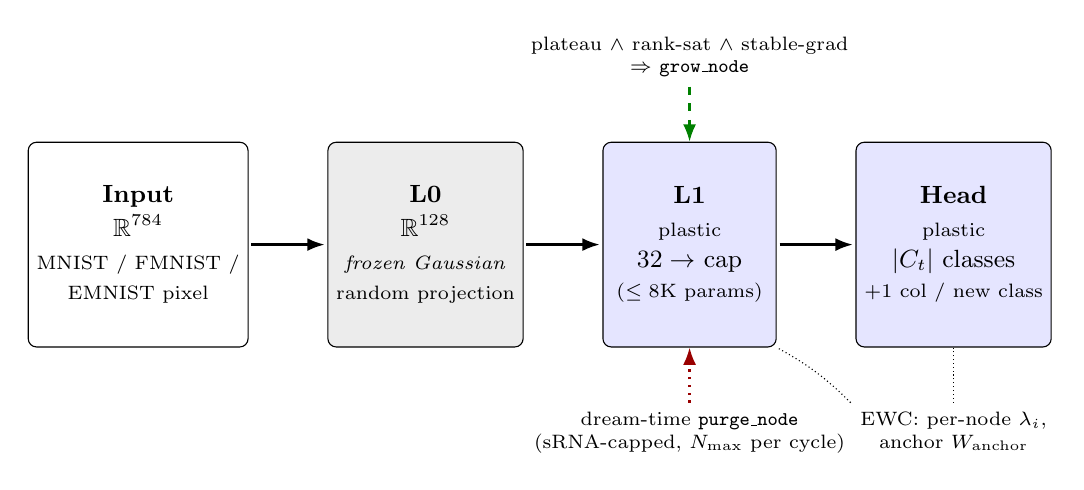
\begin{tikzpicture}[
  >={Latex[length=2.2mm]},
  font=\small,
  layer/.style={draw, rounded corners=3pt, minimum width=22mm,
                minimum height=26mm, align=center, inner sep=3pt, fill=white},
  frozen/.style={layer, fill=gray!15},
  plastic/.style={layer, fill=blue!10},
  ann/.style={font=\scriptsize, align=center},
  arr/.style={->, thick, shorten >=1pt, shorten <=1pt}
]
\node[layer] (in) {\textbf{Input}\\[1pt]$\R^{784}$\\[1pt]
                   \scriptsize MNIST / FMNIST /\\\scriptsize EMNIST pixel};
\node[frozen, right=10mm of in] (l0) {\textbf{L0}\\[1pt]$\R^{128}$\\[1pt]
                   \scriptsize \emph{frozen Gaussian}\\
                   \scriptsize random projection};
\node[plastic, right=10mm of l0] (l1) {\textbf{L1}\\[1pt]
                   \scriptsize plastic\\$32 \to$ cap\\
                   \scriptsize ($\le 8\text{K}$ params)};
\node[plastic, right=10mm of l1] (hd) {\textbf{Head}\\[1pt]
                   \scriptsize plastic\\$|C_t|$ classes\\
                   \scriptsize +1 col / new class};
\draw[arr] (in) -- (l0);
\draw[arr] (l0) -- (l1);
\draw[arr] (l1) -- (hd);
\node[ann, above=7mm of l1] (gtrig) {plateau $\wedge$ rank-sat $\wedge$ stable-grad\\
                                     $\Rightarrow$ \texttt{grow\_node}};
\draw[->, dashed, thick, green!50!black] (gtrig.south) -- (l1.north);
\node[ann, below=7mm of l1] (purge) {dream-time \texttt{purge\_node}\\
                                     (sRNA-capped, $N_{\max}$ per cycle)};
\draw[->, dotted, thick, red!60!black] (purge.north) -- (l1.south);
\node[ann, below=7mm of hd] (ewc) {EWC: per-node $\lambda_i$,\\
                                   anchor $\anchorW$};
\draw[densely dotted] (ewc.north) -- (hd.south);
\draw[densely dotted] (ewc.north west) to[bend right=8] (l1.south east);
\end{tikzpicture}
\caption{Base trioron architecture for chained-15. The frozen Gaussian
L0 projection provides a stable code space for manifold replay
(\S\ref{sec:manifold-replay}). The plastic L1 grows under the
conjunction of loss-plateau, rank-saturation, and gradient-stability
triggers up to a per-curriculum byte cap; the head grows one column
per new class. Dream-time purge removes low-utility nodes, gated by
the per-cycle event cap (\S\ref{sec:srna-cap}). EWC anchors plus
per-node plasticity $\lambda_i$ pin prior-task knowledge on plastic
layers.}
\label{fig:trioron-arch}
\end{figure}

\subsection{The Frustration Multiplier}
\label{sec:frustration}

We add a per-task plateau counter that scales the task loss when the
optimizer gets stuck. For each task we accumulate the loss in windows
of length $W_f$. At each window boundary we compare this window's mean
loss to the prior window's; if improvement is below $\varepsilon_f$, we
increment a stuck counter $s$. The multiplier is
\begin{equation}
  m = \min(M_{\max},\; 1 + g \cdot \max(0, s - \tau + 1)),
\end{equation}
with hinge threshold $\tau$, gain $g$, and ceiling $M_{\max}$. The
multiplier is applied \emph{only to the task loss}, not the EWC
penalty:
\begin{equation}
  L = m \cdot \Ltask + \beta \cdot \Lewc.
\end{equation}
This is mechanically equivalent to focal-loss / hard-example mining:
amplify the gradient signal on examples the optimizer is not
progressing on, without amplifying the regularizer. The biological
analogue we have in mind is the HPA-axis stress response: sustained
behavioral failure to make progress elevates glucocorticoids, which
modulate plasticity-related gene expression through epigenetic
mechanisms. The frustration multiplier is the architecture's
stress-proxy switch; we do not claim it reproduces the biology.

\subsection{The Dreaming Phase}
\label{sec:dreaming-phase}

Between training tasks we run an offline \emph{dreaming block}: a short
sleep-time pass that consolidates what was just learned without
exposing the network to new data. Frustration is disabled inside the
dream block (no environmental stress during sleep); EWC remains active
so that consolidation pulls weights toward their anchored state. The
dream block runs four sequential stages:
\begin{equation*}
  \text{replay} \;\to\; \text{compression (optional)} \;\to\;
  \text{purge} \;\to\; \text{archive}.
\end{equation*}
Replay (\S\ref{sec:replay}) is the load-bearing accuracy mechanism;
the dream archive (\S\ref{sec:archive}) is the load-bearing storage
mechanism; compression is documented as an ablation arm
(\S\ref{sec:compress-arms}); purge is gated by a per-cycle event cap
(\S\ref{sec:srna-cap}).

\subsubsection{Replay}
\label{sec:replay}

Replay rehearses past tasks under EWC. We support two replay sources:
\begin{itemize}[leftmargin=1.5em]
  \item \emph{Episodic exemplars (hippocampal buffer).} When real-data
        storage is permitted we maintain a buffer of $K$ samples per
        past task, sampled uniformly at task end. During replay the
        buffer is shuffled with the current task's batch (1{:}1 by
        default) and the cross-entropy loss is evaluated on both.
        $K \in \{1, 10, 20, 50\}$ is the storage axis we sweep in
        \S\ref{sec:pareto}. $K = 0$ routes replay through the
        storage-free pseudo-rehearsal pathway of
        \S\ref{sec:manifold-replay}.
  \item \emph{Manifold pseudo-rehearsal (storage-free).} Per-class
        statistics of L0 activations are stored at task end and used
        to synthesize replay samples; see \S\ref{sec:manifold-replay}
        for the full mechanism.
\end{itemize}
Conceptually analogous to sharp-wave ripples during slow-wave sleep,
which replay recent and remote memories at compressed timescales
\citep{tononi2014sleep}.

\subsubsection{The sRNA Cap}
\label{sec:srna-cap}

Each dream block bounds the number of structural-pruning events per
layer by a per-cycle cap $N_{\max}$. The cap holds even when many
candidates pass the utility threshold of \S\ref{sec:purge}: across the
dream-time mechanism design space we explored, $\sigma$-distance from
baselines degrades monotonically with structural event count,
motivating small caps. The default in the working configuration is
$N_{\max} = 1$ --- at most one purge event per layer per dream cycle,
allowing replay to absorb the structural change before the next event
drifts on top.

The cap is a stand-in for resource-limited small-RNA pools that gate
sleep-cycle synaptic homeostasis: miRNAs involved in synaptic
remodeling are produced and consumed in stoichiometric amounts during
a single sleep cycle \citep{schratt2009micrornas, tononi2014sleep}, so
the cellular machinery cannot perform arbitrarily many remodeling
events per cycle. The ``fewer events $=$ better'' empirical pattern is
broadly consistent with that biological observation, though we do not
claim a tight quantitative match.

\subsubsection{Compression-Action Design Space (Ablation Arms)}
\label{sec:compress-arms}

Three substrate-respecting mechanisms for resolving a detected
redundant pair $(i, j)$ were tested as dream-time compression actions:
\emph{synaptic downscale} (the kept side absorbs the victim's outgoing
column, victim is zeroed, victim's row is not touched); \emph{routing
starvation} (asymmetric multiplicative ramp on the victim's routing
scale, with regrow on non-victims); and \emph{apoptosis spike} (when a
routing-starved scale crosses the floor, the dead cell's outgoing is
redistributed and surviving peers' apoptosis pulses $p_i$ are raised,
which transiently reduces their EWC stiffness via \S\ref{sec:trioron-node}).
None of these arms beats the no-compression baseline at $n = 6$ seeds
in our experiments; we document them here as the ablation arms reported
in \S\ref{sec:results}, and motivate the substrate-preserving emphasis
that motivates \S\ref{sec:archive}. Engagement statistics are bimodal:
at the activation-cosine threshold $\tau_{\ac} = 0.92$ (the redundancy
detector), about half the seeds fire zero events --- a pattern that
across-seed averaging conceals.

\subsubsection{Purge}
\label{sec:purge}

The purge stage drops nodes whose utility $u_i$ falls below a threshold
$\tau_u$, subject to the per-layer cap $N_{\max}$ of
\S\ref{sec:srna-cap}. It reuses the structural pruning machinery of
\S\ref{sec:structural-plasticity}, including cross-layer fan-in cleanup
and cosine-nearest-peer redistribution. Distinct from the in-training
pruner (\S\ref{sec:structural-plasticity}): purge is a sleep-time
structural sweep with a strict event cap, not an event-clock check
during waking training.

\subsubsection{Pseudo-code of a Dream Block}
\label{sec:dream-pseudocode}

\begin{verbatim}
for each task t in curriculum:
    train_one_task(t)                         # waking
    consolidate_task(t)                       # Fisher update + anchor
    if dreaming_enabled:
        decay apoptosis pulses by delta
        replay(buffer = hippo or manifold,
               steps = K_r,
               ewc_active = True)
        compress(signal = activation,
                 threshold = tau_ac,
                 action = ACTION,            # ablation arm; default off
                 max_events_per_layer = N_max)
        purge(threshold = tau_u)
        archive_block(...)                    # see archive section
\end{verbatim}

\subsection{Manifold Replay (Storage-Free Pseudo-Rehearsal)}
\label{sec:manifold-replay}

The headline rehearsal mechanism is \emph{manifold replay}: a
trioron-native pseudo-rehearsal scheme that summarizes each past class
as a small set of statistics in the network's first-hidden-layer (L0)
representation rather than storing exemplars.

\paragraph{Storage.}
When a task $t$ ends we collect L0 activations for each class $c$ that
appeared in the task and store the per-class mean
$\mu_c \in \R^{L_0}$ and per-dimension standard deviation
$\sigma_c \in \R^{L_0}$ (a diagonal-Gaussian summary). Storage per
class is $2 \cdot L_0 \cdot 4 = 1024$ bytes at $L_0 = 128$. A 30-class
run costs $\approx\!30$~KB total --- independent of the dataset size
and of the number of samples per task.

\paragraph{Replay.}
During the dream block we draw pseudo-samples for each past class $c$:
\begin{equation}
  \tilde z = \mu_c + \sigma_c \odot \varepsilon,
  \qquad \varepsilon \sim \mathcal{N}(0, I),
\end{equation}
then forward them through the \emph{upper} layers via
\texttt{forward\_from\_layer(z\_tilde, start = 1)} to obtain logits.
Cross-entropy loss on $(\tilde z, c)$ is added to the total loss.
Replay is performed at the same EWC strength as waking training.

\paragraph{Why per-class statistics work where logit-inversion fails.}
Three single-seed inversion variants ---
DeepInversion-style code synthesis \citep{yin2020deepinversion}
(one-shot, refresh-all, and diversity-regularized) --- all peaked at
$0.27$ full-softmax accuracy on chained-15. Logit inversion locates
class-$c$ attractor \emph{peaks}, not class-$c$ manifold
\emph{samples}; the resulting points concentrate at adversarial extrema
that do not reflect actual class structure. The $(\mu, \sigma)$ summary
lives on the real L0 manifold by construction; inversion attractors do
not. An ablation removing per-class $\sigma$ ($\mu$-only replay) loses
$\approx\!0.07$ absolute on full-softmax at 30 classes (single seed),
suggesting that per-class noise scale is load-bearing --- roughly
$12\%$ of manifold replay's advantage.

\paragraph{Why L0 is frozen.}
Manifold replay assumes that L0's encoding is approximately stationary
across the curriculum, so that statistics collected after task $t$
remain valid at task $t + k$. We enforce this by freezing L0 at
initialization to a fixed random Gaussian projection (weights drawn
from $\mathcal{N}(0, 2/d)$ at init and never updated). A
separation-probe diagnostic on the chained-15 curriculum gives a
class-prototype discriminability ratio of $1.063$ in the frozen L0
space --- modest but non-trivial, with Fashion-MNIST contributing the
lowest separability ($1.04$) as expected from its irreducible
within-domain confusions. The ratio rules out a single-prototype
scheme (L0-space class means alone are not separable enough) and
motivates the stored-$(\mu, \sigma)$ sketch as a manifold summary
rather than a class-prototype classifier.

\paragraph{Epigenetic analogue.}
Per-class $(\mu, \sigma)$ is a compact ``engram fingerprint'': an
offline sketch of the data manifold rather than a stored sample.
Functionally closer to consolidated memory traces (gist-level recall)
than to episodic exemplar storage (which the hippocampal-buffer
baseline of \S\ref{sec:replay} implements explicitly).

\subsection{The Dream Archive}
\label{sec:archive}

Long curricula accumulate parameters that should not keep moving ---
rows whose Fisher has plateaued and whose contribution is stable across
recent tasks. We expose these as a \emph{dream archive}: a two-phase
mechanism for locking and quantizing such rows.

\paragraph{Phase 1 --- mid-curriculum row archive.}
After each \texttt{consolidate\_task}, every row of every layer is
scored along three axes: (a) $\lambda$ percentile (top
\textit{archive\_lam\_top\_percentile} of the layer), (b)
gradient-magnitude ceiling (median $|g|$ over the recent window below
\textit{archive\_grad\_mag\_floor}), and (c) apoptosis-pulse bound
($p \leq$ \textit{archive\_pulse\_max} --- never archive a row recently
pulsed by an apoptosis event). A row that satisfies all three for
\textit{archive\_streak\_threshold} consecutive tasks is
\emph{archived}: a per-row gradient mask is set so subsequent backward
passes leave the row at its anchor value. The mask is enforced via
\texttt{mask\_archived\_grads\_all()} between \texttt{loss.backward()}
and \texttt{opt.step()} (sequenced after PackNet/HAT grad surgery on
competitor arms). A per-layer cap \textit{archive\_max\_per\_layer}
prevents any one layer from being fully archived in a single pass.

\paragraph{Phase 2 --- end-of-curriculum int8 quantization.}
At end of training we snap each archived row to int8 with a per-row
symmetric scale ($8$~bits/weight plus one fp32 scale per row). Active
(non-archived) weights are rounded to BF16 precision. The Phase 2 path
is implemented as a snapshot--quantize--re-evaluate--restore sequence
in the bench so we can report storage and accuracy numbers from the
same trained checkpoint; the deployment path applies the snap
permanently.

\paragraph{Storage accounting.}
With BF16 as the deployment baseline, archive $+$ int8 reduces network
weight storage by $\approx\!40\%$ across all arms ($213.7 \to
127.5$~KB on the headline \arm{grown\_capped\_dream} arm; full table
in \S\ref{sec:archive-results}). We report deployment storage in the
BF16 baseline because that is the honest device-side accounting; an
FP32 baseline overstates the dream-archive win.

\paragraph{Why ternary fails on a frozen-L0 substrate.}
Ternary quantization ($2$~bits/weight) on the frozen-Gaussian L0
projection costs $0.31$ absolute full-softmax accuracy on the smoke
test: random-Gaussian weights have no concentration of magnitude near
zero, so $2$-bit quantization throws away most of the routing
structure that L1 and the head learned to depend on. Int8
($\approx 1/127 \approx 0.8\%$ per-weight noise) preserves the routing
intact. Unlocking ternary would require quantization-aware training
during the dream phase, or restricting ternary to layers whose weights
are concentrated at zero (a learned, pruned L1 + head) --- both
deferred to future work.

\paragraph{Epigenetic analogue.}
Phase 1 is a stand-in for terminal cell differentiation --- a cell
that has settled into its mature role no longer participates in
plasticity. Phase 2 is a stand-in for compression of consolidated
memory traces into low-bandwidth long-term storage, freeing
high-bandwidth substrate for new learning.

\subsection{Mixed-Precision Substrate}
\label{sec:mixed-precision}

For deployment on resource-constrained devices the architecture
supports a mixed-precision mode in which weight Parameters $(W, b)$
are stored in narrow precision (BF16) while all consolidation buffers
--- $\anchorW, \anchorB, F_W, F_b, \lambda, u, r, p$ --- remain in
FP32. The forward pass auto-casts inputs to the weight dtype,
preserving the callable interface; the EWC penalty and Fisher
accumulation upcast cleanly across the boundary.

This separation is necessary: pure-narrow-precision training degrades
by $\approx\!40\%$ due to optimizer-state precision loss in Adam's
running moments, but inference latency and memory cost are dominated
by the weights, which can safely run in BF16. The intended deployment
pattern is \emph{train in FP32 during sleep cycles, deploy in BF16 for
always-on inference}.

\subsection{The Ship-Wake-Extend Loop}
\label{sec:ship-wake-extend}

Deployment is not a one-shot training run that yields a fixed
artifact; it is an iterative loop in which the model is shipped, woken
on new data, allowed to grow plastic substrate, and re-shipped. We
instantiate this loop with a \emph{consolidation-dream pass} that
fires once at a chosen task boundary:
\begin{enumerate}[leftmargin=2em]
  \item \texttt{consolidation\_dream\_pass} --- full-coverage replay
        over all past tasks with archive-aware gradient masking (locks
        honored), plus one additional \texttt{archive\_block} call to
        catch rows that just settled.
  \item Optional permanent int8 snap of the archived rows (no restore
        step, since this is the shipping checkpoint).
  \item Cap lift:
        $\textit{current\_cap\_bytes} \leftarrow
         \textit{extension\_cap\_bytes}$.
        The network is allowed to grow new plastic substrate against
        the new task budget.
  \item The training loop continues over the new tasks with shared
        internal state --- manifold buffer, EWC anchors, archived
        rows, frustration counters all persist across the boundary.
\end{enumerate}

The result is a smaller plastic envelope in deployment than in
training, with new growth allocated only against the residual. A
device-conscience deployment cannot revisit the original training
data: it has only what it has stored (the manifold buffer, the
archived weights) and what arrives in the new data stream. The
consolidation-dream pass turns shipping into a controlled handoff:
the network ``sleeps long'' before going to market, locking in the
rows it will never need to move again, then wakes on new data in the
field.

\subsection{Multi-Branch Absorption}
\label{sec:absorption}

The ship-wake-extend loop (\S\ref{sec:ship-wake-extend}) lets a single
organism continue learning across deployment cycles. A natural next
question is whether two organisms trained \emph{independently} on
disjoint task streams can be \emph{composed} into a single recipient
without retraining either of them. We construct a multi-branch
organism that does so, with a shared frozen L0 random projection as
the only structural prerequisite.

\paragraph{Architecture.}
A multi-branch organism comprises a shared frozen L0 (the same
Kaiming-initialized random projection used in single-branch trioron,
\S\ref{sec:methods}) and $N$ parallel \emph{branches}. Each branch is
a self-contained donor produced by an independent training run: a
frozen L1 substrate, a frozen head slice over its own covered class
subset, and the per-class manifold archive
$\{(\mu_c, \Sigma_c)\}_{c \in C_b}$ that is already computed for
manifold replay (\S\ref{sec:manifold-replay}). The branches share the
same L0 random projection by being born at the same seed --- the
\emph{shared-seed invariant} --- which is what makes donor weights
semantically valid in recipient code-space without distillation. We
enforce non-overlap of class coverage across branches:
$C_b \cap C_{b'} = \emptyset$ for $b \neq b'$.

\paragraph{Forward pass.}
For input $x$:
\begin{enumerate}[leftmargin=2em]
  \item Project to code space:
        $z = \sigma(W_{L_0} x + b_{L_0})$ using the shared L0.
  \item For each branch $b$, compute the per-branch head logits
        $\ell^{(b)} = \text{branch}_b(z)$ over $C_b$.
  \item Compute per-branch generative log-likelihoods from the archive
        as a uniform mixture of per-class diagonal Gaussians:
        $$\log p_b(z) = \log\!\left(
          \tfrac{1}{|C_b|}
          \sum_{c \in C_b} \mathcal{N}(z;\mu_c, \Sigma_c)
        \right).$$
  \item Compute branch gates by softmax over branches:
        $$g_b(z) = \frac{\exp(\log p_b(z) / T)}
                       {\sum_{b'} \exp(\log p_{b'}(z) / T)},$$
        where $T$ is a temperature ($T = 1$ default). Soft gates
        (rather than argmax) are deliberate: when archive
        log-likelihoods on a query are close, multiple branches
        co-fire and their log-probability contributions are blended.
  \item Compose into combined logits over the union
        $C_{\cup} = \bigsqcup_b C_b$ via the principled
        mixture-of-experts log-probability:
        $$\text{combined}_c(z) = \log g_{b(c)}(z) +
          \log\text{softmax}_c(\ell^{(b(c))}),$$
        where $b(c)$ is the unique branch covering $c$.
\end{enumerate}

\begin{figure}[t]
\centering
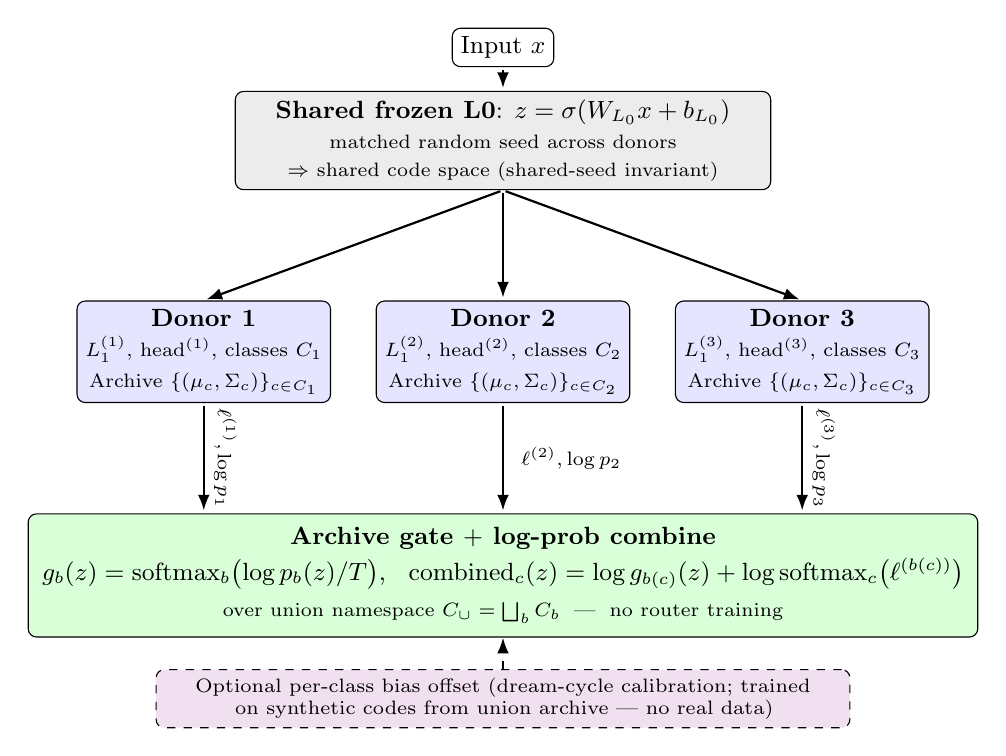
\begin{tikzpicture}[
  >={Latex[length=2mm]},
  font=\small,
  L/.style={draw, rounded corners=3pt, align=center, inner sep=3pt, fill=white},
  frozen/.style={L, fill=gray!15},
  donor/.style={L, fill=blue!10, minimum width=30mm, align=center},
  combine/.style={L, fill=green!15, minimum width=98mm, align=center, inner sep=5pt},
  bias/.style={L, dashed, fill=violet!12, font=\scriptsize, align=center},
  s/.style={font=\scriptsize, align=center},
  arr/.style={->, thick, shorten >=1pt, shorten <=1pt}
]
\node[L] (in) {Input $x$};
\node[frozen, below=3mm of in, minimum width=68mm] (l0)
  {\textbf{Shared frozen L0}: $z = \sigma(W_{L_0} x + b_{L_0})$\\
   \scriptsize matched random seed across donors\\[-1pt]
   \scriptsize $\Rightarrow$ shared code space (shared-seed invariant)};
\draw[arr] (in) -- (l0);

\node[donor, below=14mm of l0, xshift=-38mm] (d1)
  {\textbf{Donor 1}\\\scriptsize $L_1^{(1)}$, head$^{(1)}$, classes $C_1$\\
   \scriptsize Archive $\{(\mu_c, \Sigma_c)\}_{c\in C_1}$};
\node[donor, below=14mm of l0]              (d2)
  {\textbf{Donor 2}\\\scriptsize $L_1^{(2)}$, head$^{(2)}$, classes $C_2$\\
   \scriptsize Archive $\{(\mu_c, \Sigma_c)\}_{c\in C_2}$};
\node[donor, below=14mm of l0, xshift=38mm] (d3)
  {\textbf{Donor 3}\\\scriptsize $L_1^{(3)}$, head$^{(3)}$, classes $C_3$\\
   \scriptsize Archive $\{(\mu_c, \Sigma_c)\}_{c\in C_3}$};

\draw[arr] (l0.south) -- (d1.north);
\draw[arr] (l0.south) -- (d2.north);
\draw[arr] (l0.south) -- (d3.north);

\node[combine, below=14mm of d2] (cmb) {%
  \textbf{Archive gate $+$ log-prob combine}\\[2pt]
  $g_b(z) = \mathrm{softmax}_b\bigl(\log p_b(z)/T\bigr)$,\;\;
  $\text{combined}_c(z) = \log g_{b(c)}(z) +
   \log\mathrm{softmax}_c\bigl(\ell^{(b(c))}\bigr)$\\[2pt]
  \scriptsize over union namespace $C_\cup = \bigsqcup_b C_b$ \;|\; no router training};

\draw[arr] (d1.south) -- node[s, sloped, above]{$\ell^{(1)}, \log p_1$} (cmb.north -| d1);
\draw[arr] (d2.south) -- node[s, right=1mm]{$\ell^{(2)}, \log p_2$} (cmb.north -| d2);
\draw[arr] (d3.south) -- node[s, sloped, above]{$\ell^{(3)}, \log p_3$} (cmb.north -| d3);

\node[bias, below=4mm of cmb, text width=86mm]
  (bias) {Optional per-class bias offset (dream-cycle calibration;
          trained on synthetic codes from union archive --- no real data)};
\draw[->, dashed, thick] (bias.north) -- (cmb.south);
\end{tikzpicture}
\caption{Multi-branch absorption (chimera) at $N=3$ donors. All
donors share the same frozen Gaussian L0 by being born at matching
random seeds, so donor weights are byte-valid in the recipient code
space (\emph{shared-seed invariant}). Each donor contributes per-class
logits $\ell^{(b)}$ and a manifold-archive log-likelihood
$\log p_b(z)$; the same archive that serves manifold replay
(\S\ref{sec:manifold-replay}) also serves as the analytic Expert-Gate
\citep{aljundi2017expert} router. The combine operation places
per-branch log-softmax contributions into the union class namespace,
weighted by the gate --- no router training and no fusion-layer
learning. The dashed per-class bias offset is the optional
dream-cycle calibration.}
\label{fig:chimera}
\end{figure}

\paragraph{Why per-branch log-softmax.}
Each donor's head was trained under its own active-class mask, so
absolute logit \emph{magnitudes} across donors are not comparable.
Combining raw logits weighted by gates produces a biased argmax at
full-softmax. Passing each branch's logits through a log-softmax
restricted to its own coverage normalizes the contributions to a
common log-probability scale, after which the mixture combine is
well-posed. This is an inference-only fix; no parameters are added.

\paragraph{Why the mechanism is zero-shot.}
Donor weights are byte-valid in the recipient because L0 is shared
(matched random projection $\Rightarrow$ matched code distribution),
and donor logits are placed into recipient class-namespace via
per-class indexing. The gate is computed analytically from the
archive --- a generative Expert-Gate-style router
\citep{aljundi2017expert} using the manifold buffer trioron already
produces. No router training, no fusion-layer learning, no calibration
pass; pure paste-and-go.

\paragraph{Optional dream-cycle calibration.}
For deployments where the full-softmax metric is load-bearing, a tiny
additive bias offset can be trained to compensate for residual
cross-donor magnitude mismatch. We sample synthetic codes
$z \sim \mathcal{N}(\mu_c, \Sigma_c)$ from the union archive, forward
through the assembled organism, and apply cross-entropy on the global
label. We test two variants:
\begin{itemize}[leftmargin=1.5em]
  \item \emph{per-branch} ($N$ scalars): one bias broadcast uniformly
        over each donor's covered slots. Mathematically task-aware-safe
        (a uniform per-donor shift is monotonic on within-task argmax
        because active classes within a chained-15 task always belong
        to a single donor by disjoint coverage).
  \item \emph{per-class} ($|C_{\cup}|$ scalars): one bias per union
        class. Higher capacity, but \emph{can} perturb within-task
        argmax; trades a small task-aware loss for a larger
        full-softmax gain.
\end{itemize}
The dream cycle uses only the donors' own archives --- no real-data
retraining is performed.

\subsection{Experiment Design}
\label{sec:experiment-design}

\paragraph{Curriculum (chained-15).}
A 30-class class-incremental benchmark drawn from three datasets in
sequence:
\begin{itemize}[leftmargin=1.5em]
  \item 10 MNIST digit tasks (one new digit class per task);
  \item 10 Fashion-MNIST tasks (one new garment class per task);
  \item 10 EMNIST-letters tasks A..J (one new letter class per task).
\end{itemize}
Each task introduces exactly one new class. At evaluation time the
network is asked to classify across all classes seen so far
(full-softmax) or restricted to the same task or domain (task-aware,
domain-aware). The class-incremental framing forces the network to
commit to absolute class identities --- there is no task ID at
inference --- and is the standard hard regime for continual-learning
evaluation.

\paragraph{Why class-incremental, not task-incremental.}
Task-incremental benchmarks supply the task ID at inference, which
collapses the problem to learning a per-task classifier.
Class-incremental does not, and is therefore the regime where
partition-style methods (PackNet, HAT) suffer their characteristic
full-softmax collapse. Reporting class-incremental from the start
avoids confusing the comparison.

\paragraph{Extension curriculum (chained-23).}
chained-15 above, plus 8 additional EMNIST-letters tasks K..R
introduced at the extension boundary; total 23 class-incremental tasks
across 38 classes. Used only in the extension experiment of
\S\ref{sec:extension-results}.

\paragraph{Network configuration.}
\begin{itemize}[leftmargin=1.5em]
  \item Three layers: input $\to$ L0 $\to$ L1 $\to$ head.
  \item L0: $784 \to 128$, frozen-Gaussian random projection (weights
        drawn from $\mathcal{N}(0, 2/784)$ at init and never updated).
        See \S\ref{sec:manifold-replay} for why L0 is frozen.
  \item L1: $128 \to 32$ initial, grown adaptively up to
        $\textit{cap\_bytes} = 8\,\text{K}$ trainable parameters during
        chained-15, lifted to 16~K at the extension boundary.
  \item Head: $L_1\text{\_width} \to n_{\text{classes\_so\_far}}$,
        grown adaptively as new classes appear.
  \item Activations: ReLU on L1, identity on the head.
  \item Optimizer: Adam, $\text{lr} = 3 \times 10^{-3}$.
  \item Epochs: 4 per task. Loss: cross-entropy on the active label
        set.
  \item EWC strength: $\beta = 1000$ during waking and dream-replay
        (matched).
\end{itemize}

\paragraph{Trioron arms.}
\begin{itemize}[leftmargin=1.5em]
  \item \arm{fixed\_ewc\_small} --- no growth; L1 fixed at the
        chained-15 cap. Isolates the EWC $+$ manifold-replay
        contribution at matched parameters.
  \item \arm{grown\_capped\_no\_dream} --- growth under EWC, no
        dream-time consolidation. Isolates the dream contribution.
  \item \arm{grown\_capped\_dream} --- growth + dream within cap. The
        default deployment arm.
  \item \arm{grown\_uncapped\_dream} --- growth past cap with manifold
        replay. The upper-bound headline arm.
\end{itemize}

\paragraph{Competitor families (5).}
We benchmark against one method from each major continual-learning
family:
\begin{itemize}[leftmargin=1.5em]
  \item \emph{Hippocampal buffer (exemplar rehearsal).} $K$ samples
        per past class stored. $K \in \{1, 10, 20, 50\}$.
  \item \emph{PackNet} \citep{mallya2018packnet}. Iterative magnitude
        pruning with per-task masks. \emph{PackNet matched} matches
        our trainable-parameter budget; \emph{PackNet standard} uses
        the original recipe.
  \item \emph{HAT} \citep{serra2018hat}. Hard binary attention masks
        per task, gating each layer. \emph{Matched} and \emph{standard}
        variants as above.
  \item \emph{Online EWC} \citep{schwarz2018progress}. Fisher EMA
        across tasks with $\gamma = 0.95$; learning-rate and $\beta$
        tuned via grid search on the no-dream loss.
  \item \emph{LwF + EWC} \citep{li2018lwf, kirkpatrick2017overcoming}.
        Logit-distillation toward the anchored network on old-class
        columns, in addition to the EWC penalty.
\end{itemize}
We are explicit that PackNet and HAT are not designed for
class-incremental evaluation without the task-ID supplied at inference;
their full-softmax collapse on this benchmark is expected, and the
fairer comparison is the task-aware metric, on which they are
competitive (\S\ref{sec:competitor-sweep}).

\paragraph{Metrics.}
\begin{itemize}[leftmargin=1.5em]
  \item \emph{Full-softmax accuracy} (full): mean across all classes
        seen so far of top-1 accuracy with the unrestricted softmax.
        The hard class-incremental metric.
  \item \emph{Domain-aware accuracy} (domain): top-1 accuracy
        restricted to classes that share a dataset domain (digits,
        fashion, letters) with the query.
  \item \emph{Task-aware accuracy} (task): top-1 accuracy restricted
        to the classes of the \emph{task} the query belongs to. The
        right metric for trioron's deployment role of context-gated
        personalization atop a frozen LLM.
  \item \emph{Forgetting} (forget): mean across past tasks of
        (final-task accuracy on that task) $-$ (accuracy at the time
        the task was first introduced); positive values indicate
        forgetting.
  \item \emph{$\sigma$-vs-baseline}: paired-by-seed standardized
        effect size across $N = 3$ random seeds, reported alongside
        absolute $\Delta$. We are explicit that with $n = 3$ the
        $\sigma$ values can be inflated by tight per-arm seed-to-seed
        std rather than by a large absolute effect; we therefore
        report absolute $\Delta$ as the primary number and $\sigma$ as
        a secondary, with caveats.
\end{itemize}

\paragraph{Storage accounting.}
We report deployment storage in two columns: BF16 baseline (the honest
device-side number, since BF16 is the inference dtype) and FP32
baseline (the training-time number). The manifold buffer is counted at
FP32 (per-class $\mu$ and $\sigma$, $2 \cdot L_0 \cdot 4 = 1024$
bytes/class). All headline storage numbers in
\S\ref{sec:results} use the BF16 baseline.

\paragraph{Reproducibility.}
All benches run on commodity CPU. Each seed is fully deterministic
given the seed value, modulo a known torch nondeterminism in
archive-trigger timing (see \S\ref{sec:archive-results} for the v1/v2
reconciliation). Launcher scripts under \texttt{experiments/} accept
explicit seed lists; bench logs and CSVs from every reported run are
committed to the public repository.


\section{Results}
\label{sec:results}

\S\ref{sec:headline} reports the trioron-only multi-seed panel.
\S\ref{sec:competitor-sweep} ports the same protocol to five
continual-learning families and reads carefully across metrics.
\S\ref{sec:pareto} traces the storage-vs-accuracy Pareto.
\S\ref{sec:archive-results} reports the dream-archive Phase 1 + Phase
2 storage win. \S\ref{sec:extension-results} walks through the
ship-wake-extend loop end-to-end at 23 tasks.
\S\ref{sec:absorption-results} reports zero-shot multi-branch
absorption out to $N = 5$ donors. All numbers are $n = 3$ multi-seed
unless stated otherwise; absolute $\Delta$ is the primary effect-size
report and $\sigma$ is secondary.

\subsection{Manifold Replay Panel}
\label{sec:headline}

Table~\ref{tab:trioron-panel} reports the trioron arms on chained-15
with manifold replay enabled.

\begin{table}[h]
  \centering
  \caption{chained-15, $n = 3$ trioron panel.
           \headline\ marks the headline arm.}
  \label{tab:trioron-panel}
  \begin{tabular}{lccc}
    \toprule
    arm                              & full              & domain            & task              \\
    \midrule
    \arm{fixed\_ewc\_small}          & $0.585 \pm 0.002$ & $0.655 \pm 0.006$ & $0.951 \pm 0.001$ \\
    \arm{grown\_capped\_no\_dream}   & $0.577 \pm 0.011$ & $0.661 \pm 0.009$ & $0.951 \pm 0.000$ \\
    \arm{grown\_capped\_dream}       & $0.587 \pm 0.008$ & $0.657 \pm 0.009$ & $0.956 \pm 0.003$ \\
    \arm{grown\_uncapped\_dream}     & $0.604 \pm 0.003$ & $0.679 \pm 0.010$ & $0.960 \pm 0.001$\,\headline \\
    \bottomrule
  \end{tabular}
\end{table}

The upper-bound arm \arm{grown\_uncapped\_dream} reaches $0.604$ full /
$0.679$ domain / $0.960$ task on chained-15 at 30~KB of manifold-replay
storage. Forgetting is negative across all three seeds
($-0.566 \pm 0.009$ on \arm{grown\_uncapped\_dream}): past-class
accuracy increases over time after a task ends, because the manifold
replay block exposes the network to past classes throughout the
curriculum. We do not claim this behavior is unique to manifold replay
--- replay-based methods in general can produce negative-forgetting in
the right regime --- only that we measured it cleanly here.

\begin{table}[h]
  \centering
  \caption{Paired comparisons against \arm{grown\_uncapped\_dream},
           $n = 3$ paired by seed. Read $\sigma$ as a tightness
           indicator on a small sample; absolute $\Delta$ is the
           primary number.}
  \label{tab:trioron-paired}
  \begin{tabular}{llrr}
    \toprule
    comparison                                                                  & metric  & mean $\Delta$ & $\sigma$    \\
    \midrule
    \arm{fixed\_ewc\_small} vs \arm{grown\_uncapped\_dream}                     & full    & $-0.018$      & $-6.36$     \\
    \arm{fixed\_ewc\_small} vs \arm{grown\_uncapped\_dream}                     & task    & $-0.009$      & $-4.08$     \\
    \arm{grown\_capped\_no\_dream} vs \arm{grown\_uncapped\_dream}              & full    & $-0.027$      & $-3.44$     \\
    \arm{grown\_capped\_no\_dream} vs \arm{grown\_uncapped\_dream}              & domain  & $-0.018$      & $-18.14$    \\
    \bottomrule
  \end{tabular}
\end{table}

The paired margin against \arm{fixed\_ewc\_small} is $-0.018$
absolute on full-softmax, with the seed-paired std small enough to
register as $-6\sigma$. Earlier benches in a regression arena under a
hinge-contrastive loss showed growth-vs-fixed advantages of the same
sign but only $+1.0$--$1.2\sigma$; manifold replay tightened the
seed-to-seed variance more than it shifted the central tendency. The
absolute effect on full-softmax is small. We report it as a
defensible win at $n = 3$, not a strong one.

\subsection{Five-Family Competitor Sweep}
\label{sec:competitor-sweep}

Table~\ref{tab:competitor-sweep} ports the same chained-15 protocol to
five major continual-learning families, with the manifold-grown
upper-bound arm included. All results are $n = 3$ multi-seed.

\begin{table}[h]
  \centering
  \caption{chained-15 competitor sweep, $n = 3$.
           \headline\ marks family-best on a metric.}
  \label{tab:competitor-sweep}
  \small
  \begin{tabular}{llccc}
    \toprule
    family                  & method                       & full              & domain            & task              \\
    \midrule
    rehearsal (ours)        & manifold-grown $(\mu,\sigma)$ & $0.604 \pm 0.003$ & $0.679 \pm 0.010$ & $0.960 \pm 0.001$ \\
    rehearsal (exemplar)    & hippo $K = 50$               & $0.646 \pm 0.009$ & $0.699 \pm 0.012$ & $0.966 \pm 0.001$\,\headline \\
    partition               & PackNet matched              & $0.074 \pm 0.016$ & $0.202 \pm 0.028$ & $0.945 \pm 0.005$ \\
    partition               & PackNet standard             & $0.049 \pm 0.015$ & $0.140 \pm 0.037$ & $0.907 \pm 0.006$ \\
    attention-mask          & HAT matched                  & $0.132 \pm 0.011$ & $0.232 \pm 0.033$ & $0.938 \pm 0.006$ \\
    attention-mask          & HAT standard                 & $0.051 \pm 0.018$ & $0.147 \pm 0.015$ & $0.944 \pm 0.009$ \\
    online-regularization   & Online EWC $\gamma = 0.95$   & $0.187 \pm 0.033$ & $0.347 \pm 0.027$ & $0.957 \pm 0.001$ \\
    distillation            & LwF $+$ EWC                  & $0.199 \pm 0.047$ & $0.380 \pm 0.052$ & $0.964 \pm 0.001$ \\
    \bottomrule
  \end{tabular}
\end{table}

\paragraph{What the table shows.}
On full-softmax and domain-aware, manifold-grown is well above the
non-rehearsal baselines (PackNet, HAT, Online EWC, LwF$+$EWC) but
below an episodic-rehearsal buffer at $K = 50$. On task-aware, all
seven methods cluster tightly between $0.907$ and $0.966$; the spread
is $\sim$0.06 absolute and the per-arm seed std on this metric is
small (Table~\ref{tab:competitor-sweep}), so most pairwise margins are
single-digit absolute and a few $\sigma$ in the paired view. Read
carefully:

\begin{itemize}[leftmargin=1.5em]
  \item PackNet and HAT were not designed for class-incremental
        evaluation without a task-ID supplied at inference; their
        full-softmax numbers reflect that mismatch and not a deficit
        of the method on its home turf.
  \item LwF$+$EWC is competitive on task-aware (a metric that
        directly rewards within-old-class discrimination, which LwF's
        logit-distillation explicitly optimizes); manifold-grown ties
        it within $0.005$ absolute. We do not claim a task-aware
        win over LwF$+$EWC.
  \item The hippo $K = 50$ exemplar buffer beats manifold-grown by
        $0.04$ on full-softmax at $25\times$ the storage cost. On a
        Pareto axis this is the right comparison
        (\S\ref{sec:pareto}).
\end{itemize}

\begin{table}[h]
  \centering
  \caption{Paired absolute $\Delta$ of manifold-grown vs each
           competitor (positive $=$ ours wins). $\sigma$ in parentheses
           is provided for completeness; treat with $n = 3$ caveats.}
  \label{tab:paired-sigma}
  \begin{tabular}{lccc}
    \toprule
    comparison              & full $\Delta$ ($\sigma$) & domain $\Delta$ ($\sigma$) & task $\Delta$ ($\sigma$) \\
    \midrule
    vs PackNet matched      & $+0.529$ ($+31\sigma$)   & $+0.477$ ($+24\sigma$)     & $+0.015$ ($+3.4\sigma$)  \\
    vs PackNet standard     & $+0.555$ ($+47\sigma$)   & $+0.538$ ($+12\sigma$)     & $+0.052$ ($+9.8\sigma$)  \\
    vs HAT matched          & $+0.471$ ($+34\sigma$)   & $+0.447$ ($+12\sigma$)     & $+0.022$ ($+3.6\sigma$)  \\
    vs HAT standard         & $+0.553$ ($+27\sigma$)   & $+0.531$ ($+47\sigma$)     & $+0.016$ ($+1.7\sigma$)  \\
    vs Online EWC           & $+0.417$ ($+13\sigma$)   & $+0.332$ ($+14\sigma$)     & $+0.002$ ($+1.6\sigma$)  \\
    vs LwF $+$ EWC          & $+0.405$ ($+8\sigma$)    & $+0.298$ ($+6\sigma$)      & $-0.005$ ($-26\sigma$)   \\
    \bottomrule
  \end{tabular}
\end{table}

The large $\sigma$ values on the partition and attention-mask
comparisons are a consequence of very tight seed-to-seed std (e.g.\
PackNet standard's full std is $0.015$, ours is $0.003$, paired
std is small), not of a $30\times$ effect size in any standard sense.
The honest reading is: \emph{on full-softmax and domain-aware,
manifold-grown is consistently above PackNet, HAT, Online EWC, and
LwF in absolute terms, by margins between $0.30$ and $0.55$ on
class-incremental chained-15.} On task-aware, the field collapses to
a tight cluster near $0.95$, and the $\sigma$ values are too dependent
on tiny per-arm std to take seriously at $n = 3$.

\subsection{Storage-vs-Accuracy Pareto}
\label{sec:pareto}

Manifold replay's 30~KB sketch is competitive with episodic-exemplar
buffers an order of magnitude larger.
Table~\ref{tab:pareto} sweeps $K$ (samples per class stored) for the
hippocampal-buffer baseline alongside the manifold sketch. All rows
report \arm{grown\_uncapped\_dream} as the trioron arm.

\begin{table}[h]
  \centering
  \caption{Storage-vs-accuracy Pareto ($n = 3$ means).}
  \label{tab:pareto}
  \begin{tabular}{lrrr}
    \toprule
    variant                          & storage   & full    & gap to $K = 50$ \\
    \midrule
    engram $+$ diff (no rehearsal)   & 24~KB     & $0.260$ & $-0.39$         \\
    manifold $(\mu, \sigma)$         & 30~KB     & $0.604$ & $-0.04$\,\headline \\
    combined $+$ hippo $K = 10$      & 174~KB    & $0.570$ & $-0.08$         \\
    combined $+$ hippo $K = 20$      & 324~KB    & $0.601$ & $-0.05$         \\
    hippo $K = 50$                   & 750~KB    & $0.646$ & ---             \\
    \bottomrule
  \end{tabular}
\end{table}

Manifold Pareto-dominates hippo $K = 10$ on this benchmark
(cheaper \emph{and} more accurate), matches hippo $K = 20$ at one-tenth
the storage, and lands within $0.04$ absolute of $K = 50$ at
one-twenty-fifth the storage. On task-aware the gap to $K = 50$ is
$<\!1\%$.

Logit-inversion variants \citep{yin2020deepinversion} (one-shot, refresh-all,
diversity-regularized) all peaked at $0.27$ full-softmax in our
single-seed runs --- consistent with the engram-attractor pathology
that defeated earlier engram-replay variants. Per-class statistics
live on the real L0 manifold by construction; inversion attractors do
not. An ablation removing per-class $\sigma$ ($\mu$-only replay)
loses $\approx\!0.07$ absolute on full-softmax at 30 classes ---
roughly $12\%$ of manifold replay's advantage --- suggesting that
per-class noise scale is load-bearing. We label this as
\emph{suggestive evidence} rather than a confirmed result, given the
single-seed origin.

\subsection{Dream Archive Phase 1 + Phase 2}
\label{sec:archive-results}

Phase~1 (mid-curriculum row archive) and Phase~2 (end-of-curriculum
int8 quantization of archived rows $+$ BF16 active path) are
evaluated as a deployment-side compression layer atop the
manifold-grown architecture.

\begin{table}[h]
  \centering
  \caption{chained-15 with archive Phase~1 $+$ Phase~2, $n = 3$.}
  \label{tab:archive-acc}
  \begin{tabular}{lccc}
    \toprule
    arm                              & full v2           & full $\Delta$ vs no-archive & task $\Delta$ \\
    \midrule
    \arm{fixed\_ewc\_small}          & $0.572 \pm 0.004$ & $-0.013$                    & $+0.001$      \\
    \arm{grown\_capped\_no\_dream}   & $0.559 \pm 0.004$ & $-0.019$                    & $-0.003$      \\
    \arm{grown\_capped\_dream}       & $0.572 \pm 0.009$ & $-0.015$                    & $+0.006$      \\
    \arm{grown\_uncapped\_dream}     & $0.617 \pm 0.004$ & $+0.013$                    & $+0.006$      \\
    \bottomrule
  \end{tabular}
\end{table}

Phase~1's training-time effect lies inside seed-to-seed variance: the
same code on the same seeds produced \arm{grown\_uncapped\_dream}
$\Delta = +0.013$ in run~v2 versus $-0.004$ in run~v1, attributable
to torch nondeterminism in archive-trigger timing (task-1 accuracies
already differ before any archive fires). We do not claim Phase~1
helps or hurts during training. Phase~2 (int8 snap of archived rows
$+$ BF16 active path) is \textbf{lossless within $\Delta \leq 0.0008$}
across every arm and every seed. The BF16 $+$ int8 mixed precision
matches FP32 $+$ int8 within $\Delta \leq 0.0008$ as well.

The substantive win is on storage.

\begin{table}[h]
  \centering
  \caption{Deployment storage, BF16 baseline, $n = 3$ means.}
  \label{tab:archive-storage}
  \begin{tabular}{lrrr}
    \toprule
    arm                              & BF16 baseline & BF16 $+$ int8 archived & $\Delta$        \\
    \midrule
    \arm{fixed\_ewc\_small}          & $213.7$~KB    & $130.4$~KB             & $-39\%$         \\
    \arm{grown\_capped\_no\_dream}   & $213.7$~KB    & $128.9$~KB             & $-40\%$         \\
    \arm{grown\_capped\_dream}       & $211.2$~KB    & $127.5$~KB             & $-40\%$\,\headline \\
    \arm{grown\_uncapped\_dream}     & $224.9$~KB    & $137.2$~KB             & $-39\%$         \\
    \bottomrule
  \end{tabular}
\end{table}

Adding the 30~KB manifold buffer, the headline
\arm{grown\_capped\_dream} deployment image is $\approx 157$~KB total
(vs $241$~KB BF16-baseline $+$ manifold, $-35\%$). At an FP32
deployment baseline the same arm lands at $168$~KB FP32 $+$ int8
($-63\%$ relative), but the FP32 framing is the wrong yardstick for a
device-conscience deployment; we report BF16 throughout this work
because BF16 is the inference dtype.

The $-0.015$ full-softmax cost on \arm{grown\_capped\_dream} comes
from L1 archive, not L0: by task~15 the archive has typically locked
$32$--$49$ of L1's $48$--$92$ rows, and rows locked mid-curriculum
cannot adapt to later tasks. L0 archive is functionally a no-op (L0
is already frozen at init); locking L0 only enables the Phase~2
quantization, where most of the storage saving lives. Future work: a
more conservative L1 trigger (higher streak threshold, lower
\textit{archive\_max\_per\_layer}), or skipping L1 archive entirely
and relying on L0 quantization alone.

\subsection{Extension: Ship-Wake-Extend Loop}
\label{sec:extension-results}

We validate the full deployment loop end-to-end on a chained-15 $\to$
consolidation-dream $\to$ $+8$ EMNIST K..R curriculum (1 seed, 4
epochs/task, \arm{grown\_capped\_dream}). One-seed evidence is
documented as such.

\begin{table}[h]
  \centering
  \caption{Architecture progression across the ship-wake-extend loop
           (1 seed).}
  \label{tab:extension}
  \begin{tabular}{lcrcr}
    \toprule
    phase                & layers          & trainable    & archived             & plastic       \\
    \midrule
    start                & $(128, 32, 2)$  & $4\,194$     & $[0,\,0,\,0]$        & $4\,194$      \\
    chained-15 done      & $(128, 48, 30)$ & $7\,662$     & $[104,\,32,\,0]$     & $3\,534$      \\
    chained-23 done      & $(128, 80, 46)$ & $14\,046$    & $[128,\,40,\,0]$     & $8\,886$      \\
    \bottomrule
  \end{tabular}
\end{table}

The plastic envelope more than doubles during extension
($3\,534 \to 8\,886$ trainable parameters), allocated against the new
task budget --- but the archived rows from chained-15 are honored
throughout. The total stored network grows by $\approx 2.5\times$
while task coverage grows from $30$ to $46$ classes.

\paragraph{Accuracy at 23 tasks.}
Full $= 0.521$, domain $= 0.693$, task $= 0.948$. Per-phase task-aware
accuracy: MNIST $0.970$, Fashion $0.982$, EMNIST $0.927$ --- original
tasks survive through the extension at task-aware $\geq 0.93$.
Full-softmax dropped from $0.572$ (chained-15-only) to $0.521$
(chained-23): partly mechanical (46 vs 30 argmax competitors per
query, every sample now has more wrong answers to choose from),
partly real MNIST drift from extension-time growth (per-phase MNIST
full $0.752 \to 0.678$). The $-0.014$ task-aware drop is small and
is the right metric for trioron's deployment role of context-gated
personalization atop a frozen LLM.

\paragraph{Deployment storage} (BF16 baseline).
$121.3$~KB network (L0 $= 98.8$, L1 $= 15.3$, head $= 7.3$) plus
$\approx\!47$~KB manifold buffer (46 classes $\times$ 256 floats)
$\approx \mathbf{168}$~KB total --- $+11$~KB over the chained-15
deployment for 8 additional task capabilities.

\paragraph{Limits.}
This is one seed. Full-softmax on this cohort is also data-bounded:
per-dataset MLP joint-training upper bounds are MNIST $\approx 98\%$,
Fashion-MNIST $\approx 92$--$93\%$, EMNIST-letters $\approx
91$--$92\%$, with a combined 46-class weighted ceiling of
$\approx 0.927$. Genuine class confusions (T-shirt / shirt /
pullover; I / L; O / Q; B / 8) make $99.9\%$ full-softmax unreachable
on this benchmark at any parameter count under an MLP head, and we do
not promise it. The defensible claim is: \emph{$0.95+$ task-aware on
23 class-incremental tasks at $\approx 168$~KB total deployment,
with on-device continual learning capability across deployment
cycles}.

\subsection{Multi-Branch Absorption}
\label{sec:absorption-results}

Extension within a single organism (\S\ref{sec:extension-results})
shows the architecture supports continual learning across deployment
cycles. Multi-branch absorption asks the next question: can two
organisms trained \emph{independently} on disjoint task streams be
\emph{composed} into a single recipient with no retraining of either?
With the shared-L0 invariant (\S\ref{sec:absorption}) this is
paste-and-go.

\paragraph{Setup.}
Donors are produced by separate runs of the same
\arm{grown\_uncapped\_dream} arm at L0 seed $42$ on disjoint
chained-15 / chained-extension sub-blocks: \arm{digits} (MNIST,
classes $0$--$9$), \arm{fashion} (Fashion-MNIST, $10$--$19$),
\arm{emnist} (EMNIST $A$--$J$, $20$--$29$), \arm{emnist\_kt} (EMNIST
$K$--$T$, $30$--$39$), \arm{emnist\_uz} (EMNIST $U$--$Z$ partial,
$40$--$45$). Each donor reaches its own task-aware ceiling. We
assemble a recipient organism by loading branches in increasing-$N$
prefixes, evaluating on the union test set under \emph{soft +
per-branch log-softmax} routing.

\paragraph{Lossless task-aware out to $N = 5$.}
Donor-standalone task-aware accuracy (averaged over the donors in the
prefix) is the upper bound; the assembled organism matches it within
$\Delta \leq 0.0002$ at every $N$ tested.

\begin{center}
\begin{tabular}{rcccc}
\toprule
$N$ & upper bound (TA) & organism (TA) & gap & full-union \\
\midrule
$1$ & $0.9809$ & $0.9809$ & $+0.0000$ & $0.6910$ \\
$2$ & $0.9823$ & $0.9823$ & $+0.0000$ & $0.6099$ \\
$3$ & $0.9695$ & $0.9695$ & $+0.0000$ & $0.5314$ \\
$4$ & $0.9624$ & $0.9624$ & $+0.0000$ & $0.4716$ \\
$5$ & $0.9616$ & $0.9618$ & $+0.0002$ & $0.4462$ \\
\bottomrule
\end{tabular}
\end{center}

A bleed-flip point where soft-routing bleed flips from additive to
destructive as branches multiply did not appear at $N = 5 / 46$
classes on chained-$15$-scale data. The actual limit at this scale is
dataset variety; we ran out of disjoint class blocks within MNIST
$\cup$ Fashion-MNIST $\cup$ EMNIST. We do not claim the lossless
property holds at larger $N$ or on different data.

\paragraph{Bleed manifests where you'd predict, but does not damage
task-aware.} Diagnostic mean per-branch gate weight per task at
$N = 5$:

\begin{center}
\begin{tabular}{lrrrrr}
\toprule
task (true branch) & \arm{digits} & \arm{fashion} & \arm{emnist} & \arm{emnist\_kt} & \arm{emnist\_uz} \\
\midrule
\texttt{mnist\_0\_1} (\arm{digits}) & $0.81$ & $0.00$ & $0.03$ & $0.14$ & $0.02$ \\
\texttt{mnist\_4\_5} (\arm{digits}) & $0.74$ & $0.03$ & $0.05$ & $0.16$ & $0.03$ \\
\texttt{fashion\_0\_1} (\arm{fashion}) & $0.01$ & $0.97$ & $0.01$ & $0.01$ & $0.00$ \\
\texttt{emnist\_8\_9} (\arm{emnist}) & $0.49^*$ & $0.02$ & $0.48^*$ & $0.01$ & $0.00$ \\
\bottomrule
\end{tabular}
\end{center}

Digit inputs pull up to $0.16$ gate weight on \arm{emnist\_kt} ($O$
resembles $0$, $S$ resembles $5$ in code space). EMNIST letters
$I, J$ yield a near-$50/50$ digits/emnist gate split (starred). Yet
task-aware accuracy on \texttt{emnist\_8\_9} stays at $0.9244$,
identical to donor-standalone, because per-branch log-softmax pushes
non-covered slot contributions to $-\infty$ in log-probability space.
Soft-routing bleed is benign under principled composition on this
benchmark.

\paragraph{Comparison vs Branch-Train-Merge family ($N = 3$).}
We benchmark against two BTM variants on the same donors, replicating
both the parameter-averaging and learned-router lines of the BTM /
Branch-Train-Mix family \citep{li2022btm, sukhbaatar2024btx}.

\begin{center}
\begin{tabular}{lcccc}
\toprule
method & zero-shot & task-aware & full-union & training cost \\
\midrule
donor-standalone (upper bound) & --- & $0.9695$ & --- & --- \\
\textbf{Ours} (archive route, soft+norm) & \ding{51} & $\mathbf{0.9695}$ & $0.5314$ & $0$ \\
BTM-avg (param averaging) & \ding{51} & $0.7396$ & $0.0845$ & $0$ \\
BTM-MoE (learned router, soft+norm) & \ding{55} & $\mathbf{0.9695}$ & $0.5610$ & $400$ steps \\
BTM-MoE (learned router, raw) & \ding{55} & $0.9695$ & $0.1725$ & $400$ steps \\
\bottomrule
\end{tabular}
\end{center}

BTM-avg averages L1 substrate across donors entry-wise; the resulting
hidden units are the mean of three different feature detectors and
none of the donors' specialty features survive --- $-0.23$ absolute
task-aware here, which replicates the documented BTM-avg weakness.
BTM-MoE substitutes our archive-likelihood gate with a learned MLP
router trained $400$ steps on \texttt{(L0(x), branch\_id)} pairs from
each donor's training images; it ties our task-aware exactly at the
upper bound but requires the router-training pass on real data.

\paragraph{Dream-cycle calibration as a tunable knob.}
For deployments where full-softmax is load-bearing, a tiny additive
bias offset trained on synthetic samples drawn from each branch's
archive (no real data, no L1 retraining) closes most of the
calibration gap.

\begin{center}
\begin{tabular}{lcrrr}
\toprule
variant & params & $\Delta$ task-aware & $\Delta$ full-union \\
\midrule
no calibration (baseline) & $0$ & --- & --- \\
per-branch bias (lr=$5e\!-\!2$, $400$ st) & $3$ & $+0.0000$ & $+0.0018$ \\
per-class bias (lr=$5e\!-\!3$, $200$ st) & $30$ & $-0.0005$ & $+0.0047$ \\
per-class bias (lr=$5e\!-\!2$, $400$ st) & $30$ & $-0.0021$ & $+0.0245$ \\
\bottomrule
\end{tabular}
\end{center}

The per-branch knob is mathematically task-aware-safe (one uniform
per-donor shift is monotonic on within-task argmax under disjoint
coverage). The per-class knob trades a small amount of task-aware for
a larger full-softmax lift, landing at full-union $0.5560$ ---
$\approx 80\%$ of the BTM-MoE level ($0.5610$) without the
router-training pass on real data. Storage cost: $30$ floats $\times$
$4$ B $= 120$ B at $N = 3$, $<\!0.03\%$ of the organism.

\paragraph{Storage at $N = 3$.}
Shared L0 = $401$~KB (fixed regardless of $N$); branch substrate
$\approx 90$~KB; archives $\approx 30$~KB. Per-skill marginal cost is
$\approx 40$~KB (substrate $+$ archive); L0 amortizes across all
branches. A device that ships with the L0 footprint already present
can absorb new skills at $\approx 40$~KB each.

\paragraph{Limits we are honest about.}
This is $N \leq 5$ on a 46-class image-classification benchmark.
LLM-scale Branch-Train-Merge benchmarks --- where BTM was originally
evaluated --- have qualitatively different dynamics in expert
specialization, gate-network capacity, and class-space size; we
make no scale-extrapolation claim. The shared-L0 invariant is a hard
prerequisite: organisms with mismatched L0 seeds require a
distillation-through-paired-codes step that we have not measured here
and which is no longer instantaneous. Saturation must exist at some
$N$; we did not find it within the data variety chained-15 supports.


\section{Conclusion}
\label{sec:conclusion}

The trioron architecture occupies a small deployment footprint with
modest sacrifices on full-softmax accuracy and is competitive on
task-aware accuracy in the class-incremental setting we tested. The
contribution is a system-level integration of established components
--- per-node EWC plasticity, capacity-expanding growth gated by a
resource budget, a stress-driven plateau detector, sleep-time replay
with a per-cycle event cap, storage-free pseudo-rehearsal in a frozen
projection space, and a two-phase row-archive plus int8 quantization
path --- coupled to a ship-wake-extend deployment loop. We do not
claim a fundamentally new continual-learning mechanism; we do claim
that the integration occupies a deployment regime
($\approx 157$--$168$~KB total) that the named baselines from the
regularization, partition, and rehearsal families were not designed
to address.

\paragraph{Future work.}
Three directions follow naturally from the limits we listed:

\begin{enumerate}[leftmargin=2em]
  \item \emph{Larger benchmarks.} Move from chained-15 / chained-23
        to standard class-incremental benchmarks (Split-CIFAR-100,
        Split-MiniImageNet) and increase $n$ to $\geq 5$ before
        reporting paired $\sigma$ values. Multi-seed reruns of the
        single-seed extension and ablation results in
        \S\ref{sec:results} are the immediate gap.
  \item \emph{Larger backbones.} Couple the trioron substrate to a
        frozen vision or language backbone in the place of the random
        L0 projection. This is the deployment story the paper points
        at (context-gated personalization atop a frozen LLM) but does
        not measure.
  \item \emph{Quantization-aware training during dream.} The
        ternary-quantization path we ruled out
        (\S\ref{sec:archive}) requires QAT during the dream phase or
        L1/head pruning before snap; both are concrete next steps.
\end{enumerate}

\paragraph{Reproducibility and artifacts.}
The full implementation, launcher scripts, bench logs, and CSVs are
released under the project repository at
\url{https://github.com/Marcrockhat/trioron-project}. A live demo
(text-to-speech routing through a multi-branch organism, plus
on-device drawing-tablet teaching path) is hosted at the project's
HuggingFace Space (\texttt{Marcrockhat/trioron-demo}). The repository
includes an end-to-end \texttt{api.extend(\dots)} entry point that
wakes a shipped checkpoint on new data and re-ships it; one tutorial
exercises this loop from a 5-digit MNIST starter through to live-learn
on a sketchpad. The intent is that other researchers can continue this
work, reproduce the headline numbers, or play with the architecture on
a small device with minimal setup.


\bibliographystyle{plainnat}
\bibliography{refs}

\end{document}
